\section{Case Study}
\label{sec.case}
This section presents a case study on the identification of genes that may respond to saline stress according to the methodology presented in section~\ref{sec. framework}. 
The RNA-seq data was obtained from GEO database
\cite{GEOAcces90:online} (accession number GSE98455). This data
corresponds to $n_0=57845$ gene expression profiles of shoot tissues
measured for both control and salt condition in $m=92$ accessions of
the Rice Diversity Panel 1, with $r=2$ biological replicates. A total
of $p=3 $ phenotypic traits are used: shoot $K^+$ content, root
biomass and shoot biomass. These traits were measured for the same
$92$ genotypes, under control and salt stress conditions, and can be
found in the supplementary information
of~\cite{campbell2017allelic}.

\subsection{Data pre-processing}

DESeq2 normalization is applied to the raw data and the biological
replicates are averaged. Genes exhibiting low variance are
identified as those with ratio of upper quantile to lower quantile
smaller than $1.5$ and are removed from the normalized data. Genes
with low expression, corresponding to those having more than $80\%$
samples with values smaller than $10$, are also removed. A total of
$n_1 = 8928$ genes are kept after this filtering process.

From the Log Fold Change matrix $L_0$, genes whose difference between
upper quantile and lower quantile greater than $0.25$ are
removed. Therefore, the resulting matrix $L_1$ contains the log ratios
of $n_2 = 8928$ genes. The logarithmic ratios of the phenotipic data,
for the $92$ accessions and the $3$ traits, is also computed.

\subsection{Co-expression network construction}

The Log Fold Change matrix $L_1$ is used to compute the corresponding
similarity matrix.  For this network, it is observed that $\beta=3$
is the smallest integer such that the $R^2 \geq 0.8
$. Figure~\ref{fig:beta} depicts the degree distribution of the
similarity matrix (left) and the degree distribution of the adjacency
matrix (right), which is the degree distribution of a scale-free
network with $R^2 = 0.8$ with $\beta = 3$.

%scale-free beta 1 y 3
\begin{figure}[htpb]
  \centering
    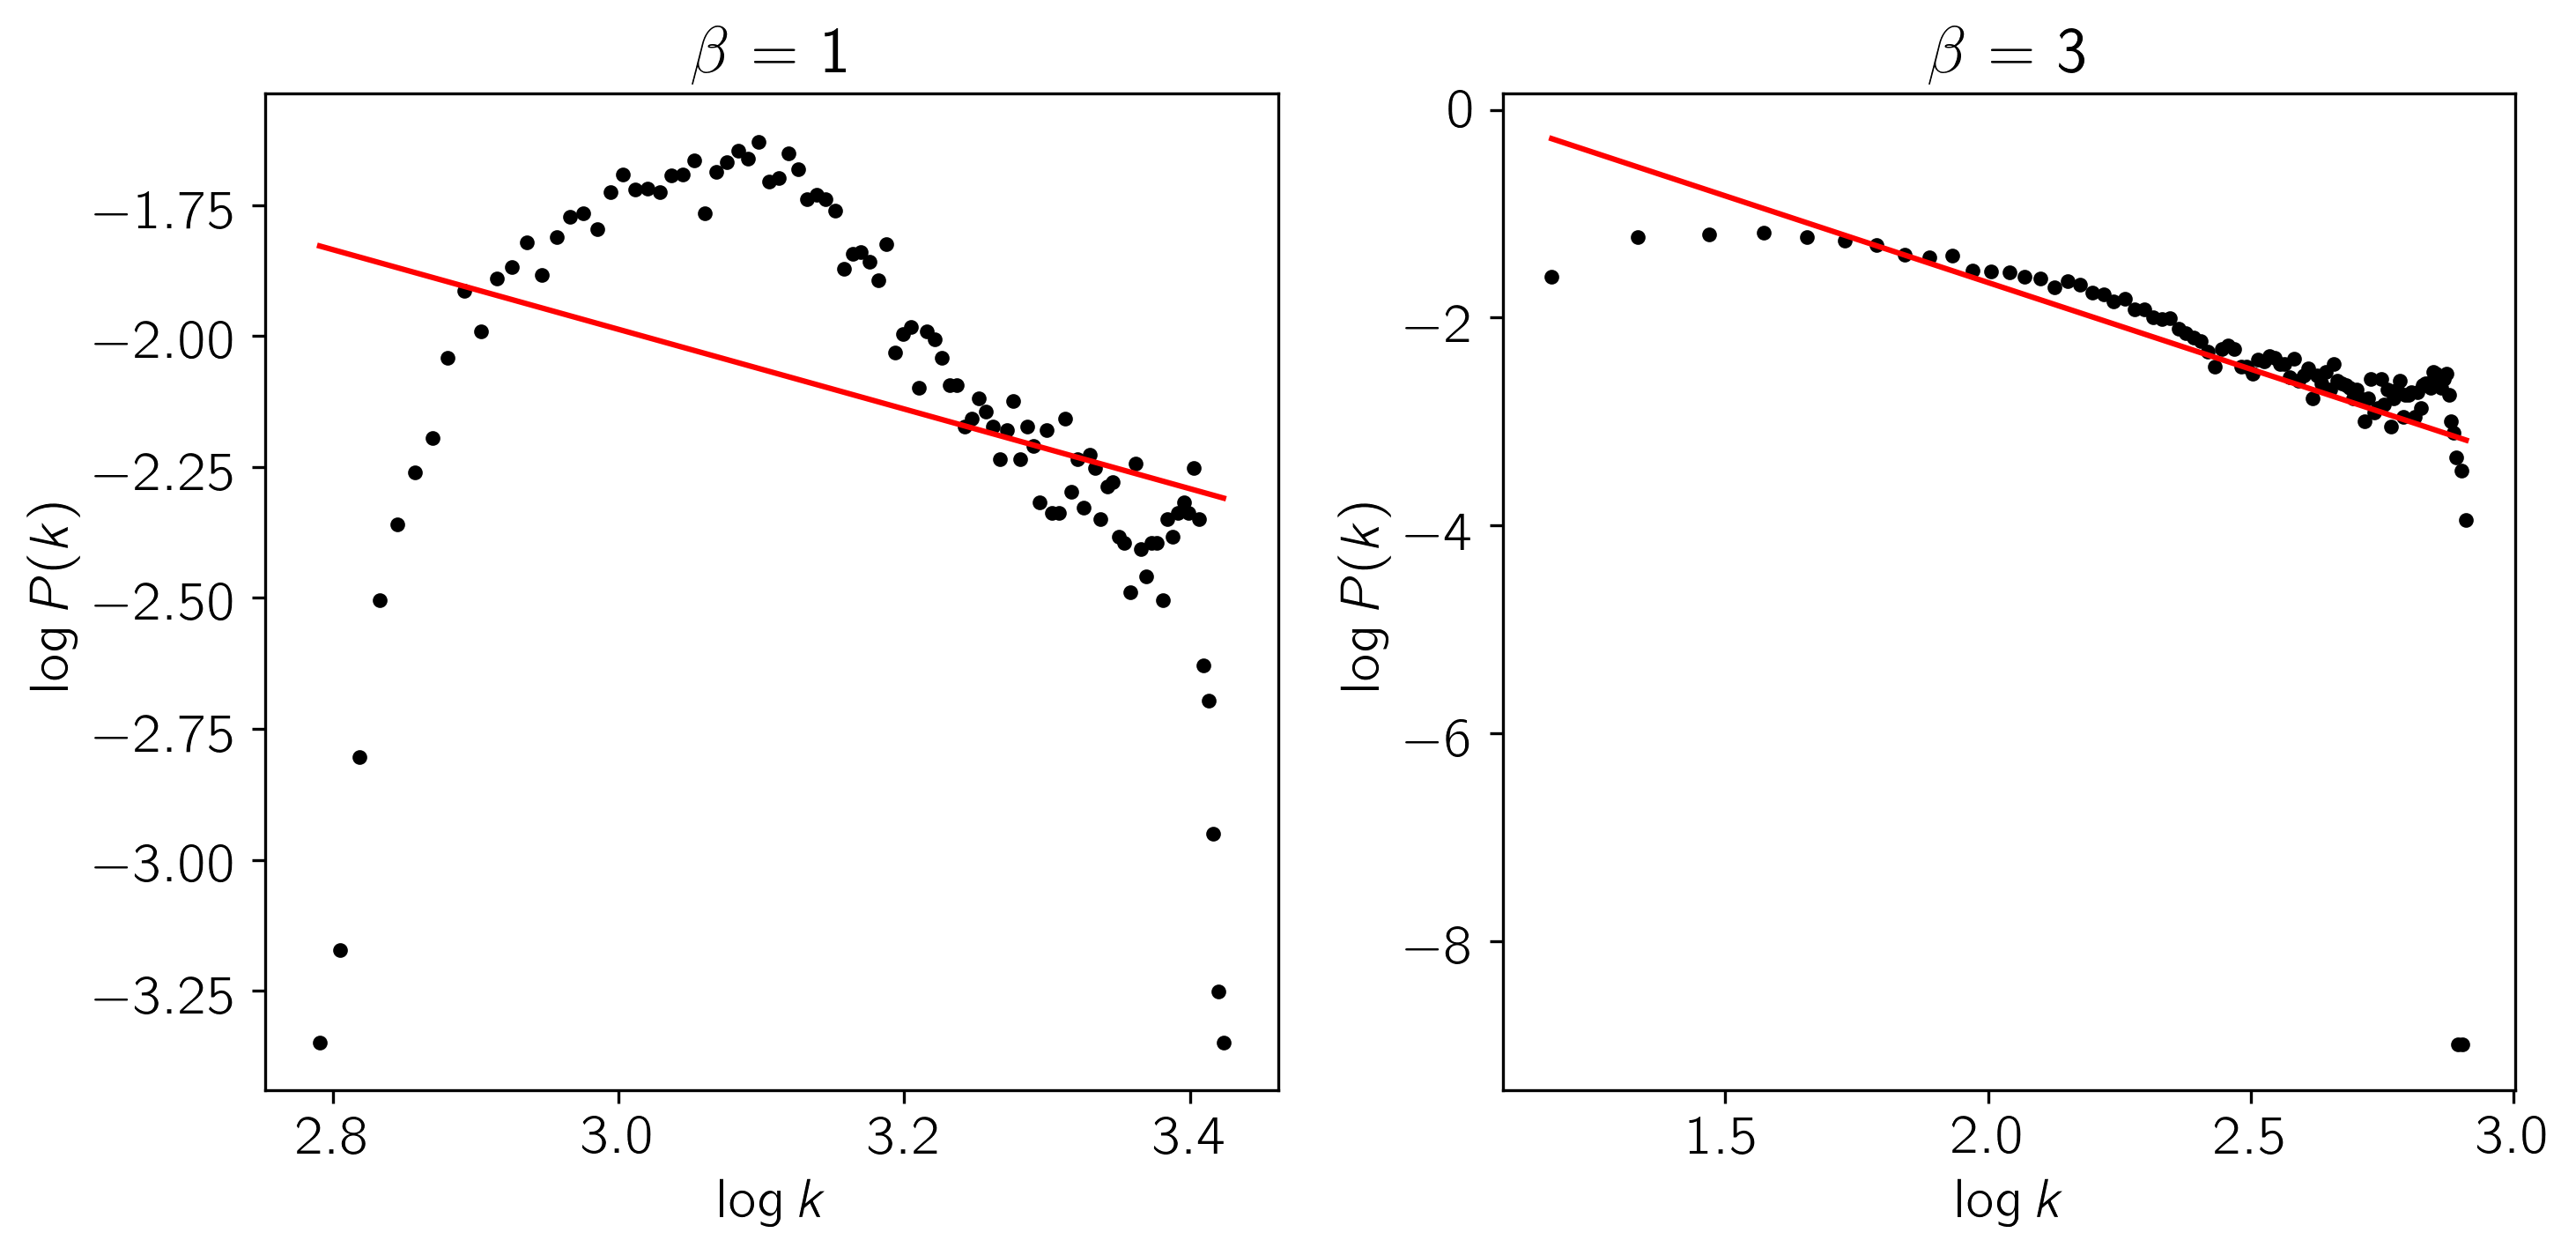
\includegraphics[clip,width=0.8\textwidth]{figures/pick_beta.png}
  \caption{Degree distribution of $A$ (left) and $\hat{A}$ (right)}
  \label{fig:beta}
\end{figure}

The resulting adjacency matrix $A$ represents a complete graph
$G=(V,E)$, with $|V| = 8928$ genes and $|E| = 39850128$ edges.

\subsection{Co-expression module identification}

The adjacency matrix $A$ is transformed into an unweighted network 
$\hat{A}$ applying the approach described in~\cite{aoki2007approaches}, 
based on the density of the network combined with the decreasing number
of nodes and edges with higher PCC values. The cutoff value is set to $0.2$,
thus keeping only the connections above this threshold and removing the 
isolated nodes. The resulting adjacency matrix $\hat{A}$ has $5810$ connected 
genes and accounts for $16875145$ edges.

After applying the HLC algorithm, a total of $4131$ genes are
distributed in $c = 5143$ overlapping modules of at least $3$ genes. Figure~\ref{fig:overlap} presents a histogram of the overlapping
percentage of these genes, measured as the proportion of modules to
which each gene belongs. The first bar of the histogram represents the
genes with zero overlap, corresponding to $28\%$ of the total
genes; remaining $72\%$ represents the genes belonging to more than one
module.

%overlapping percentage
\begin{figure}[htpb]
  \centering
    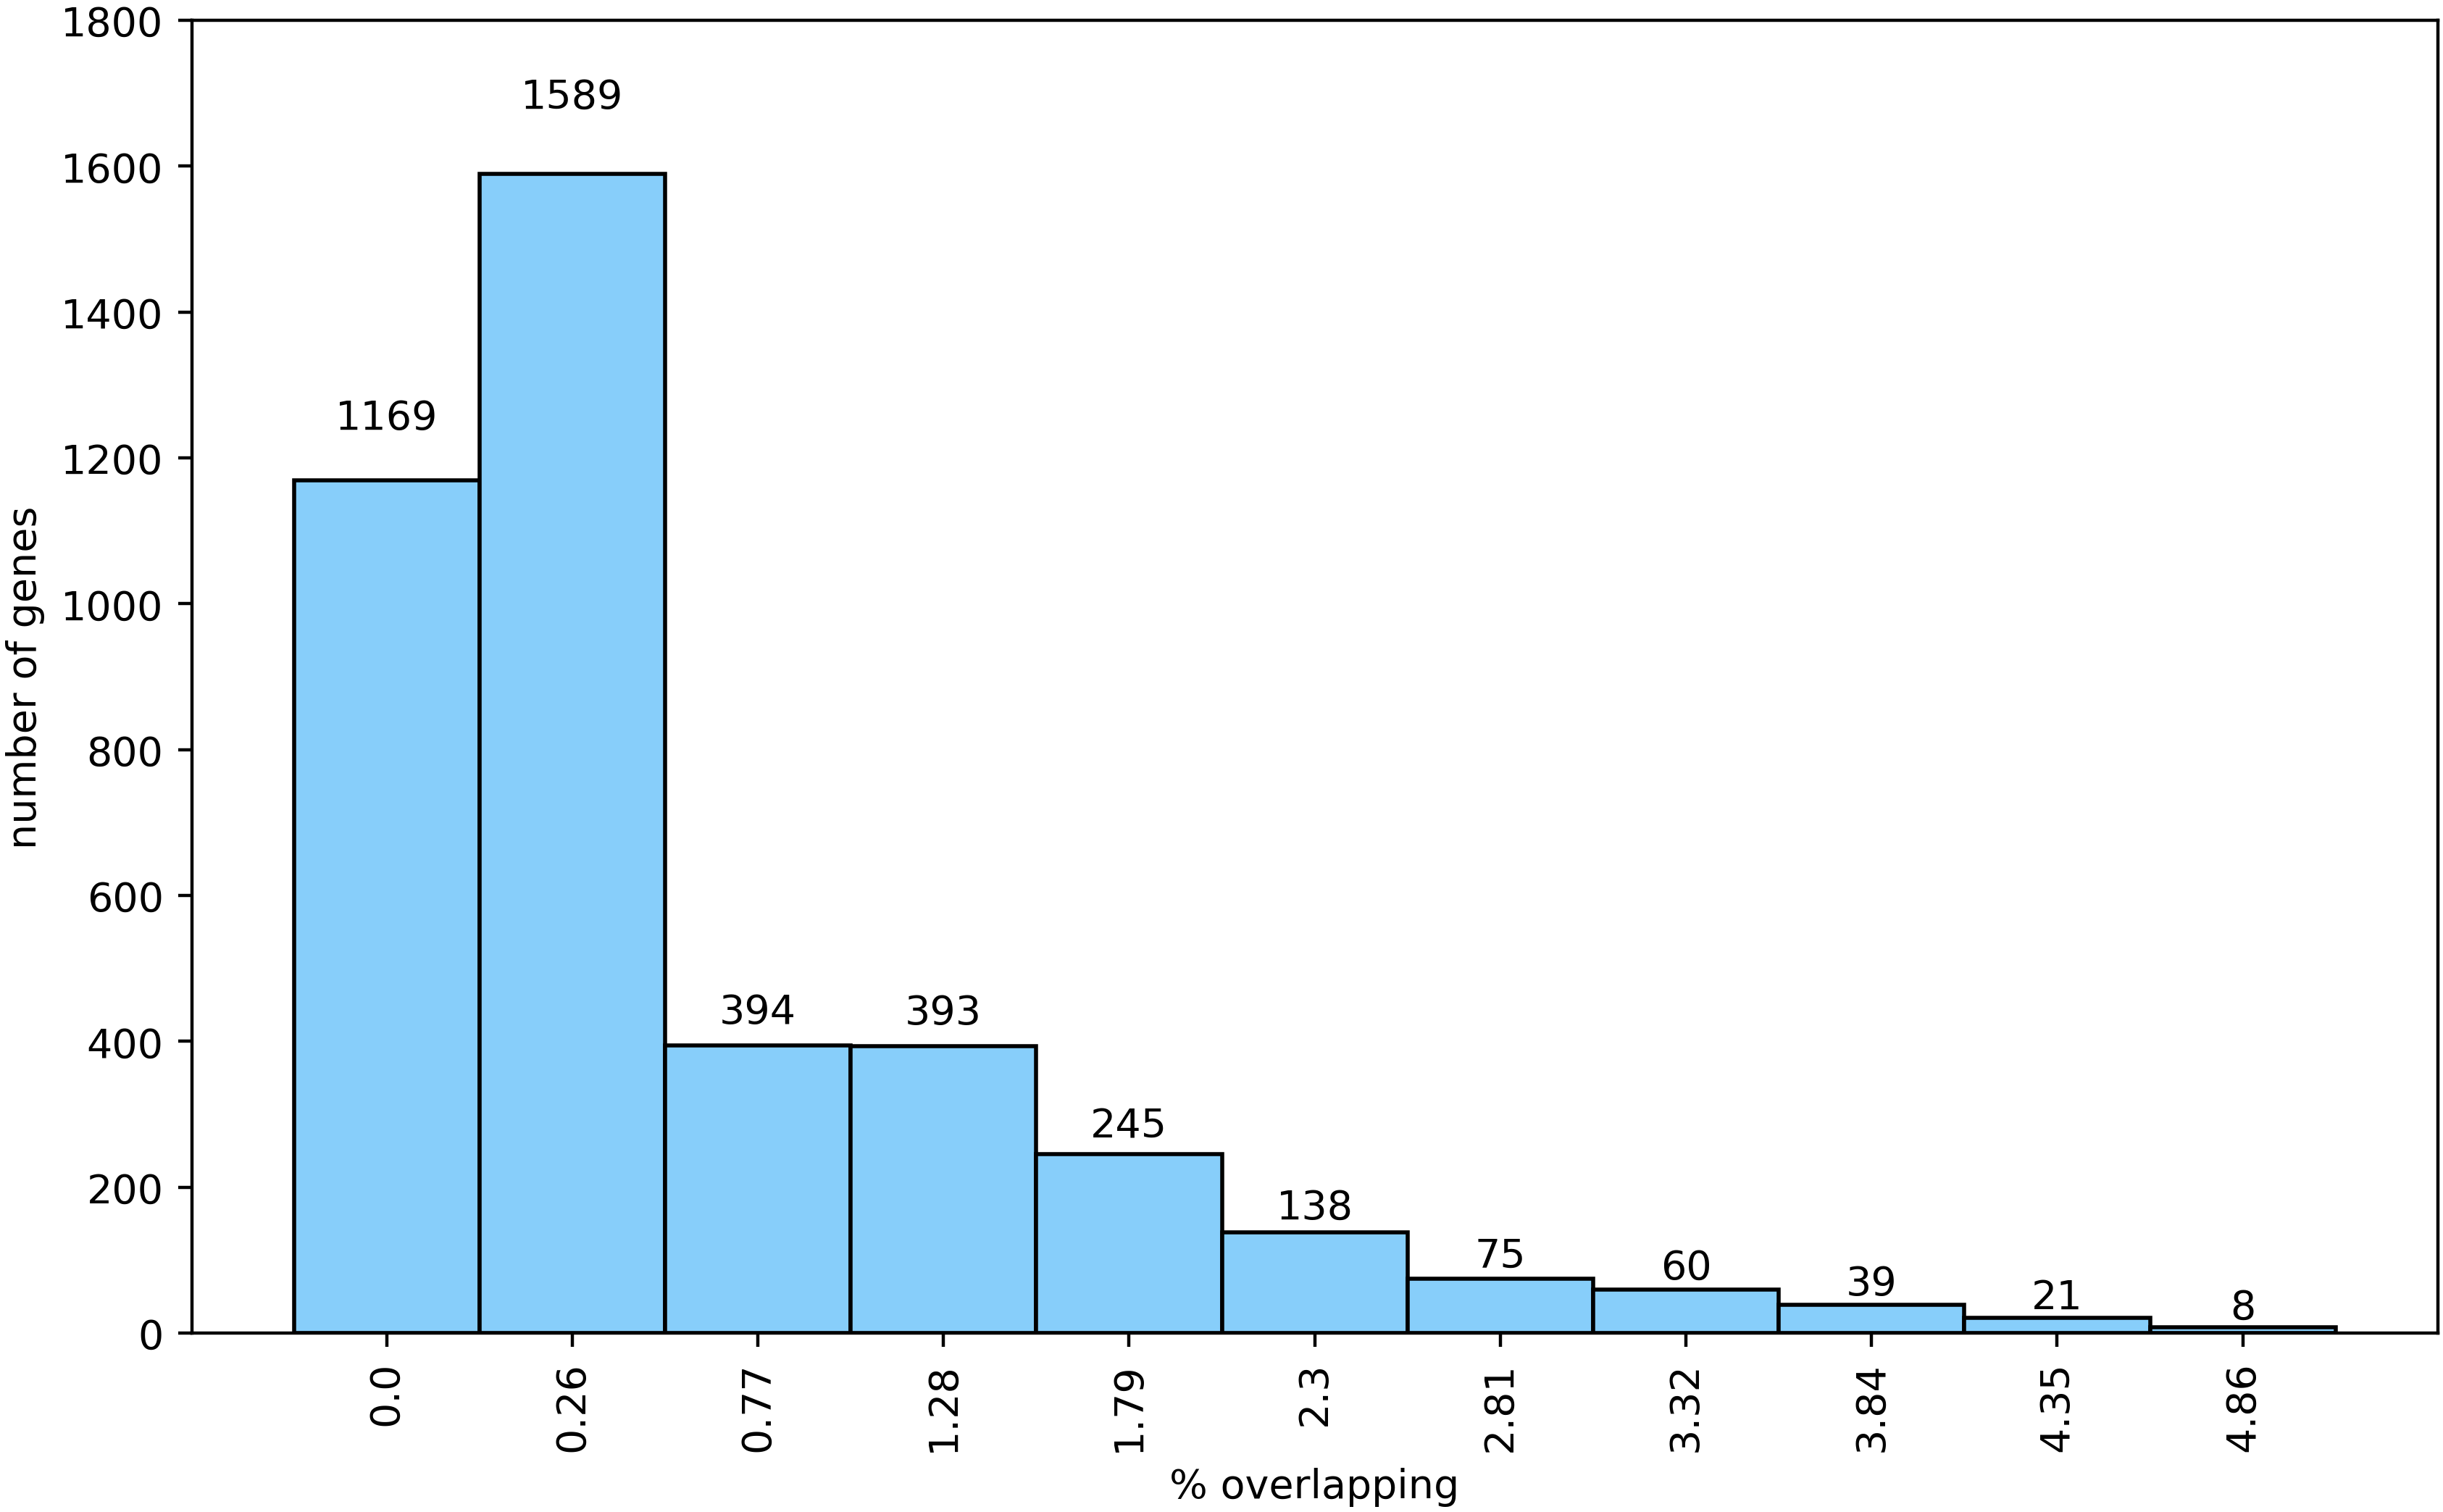
\includegraphics[clip,width=0.5\textwidth]{figures/artificial_modules.png}
  \caption{Overlapping percentage}
  \label{fig:overlap}
\end{figure}


\subsection{Module association to phenotypic traits}

The phenotypic traits under study are shoot $K^+$ content, root
biomass and shoot biomass. Figure \ref{fig:pdata} suggests that there
are significant differences in the values of these phenotypic traits
between stress and control conditions. This supports the working
hypothesis that these three variables represent tolerance-associated
traits in rice under salt stress.

% boxplots
\begin{figure}[htpb]
  \centering
    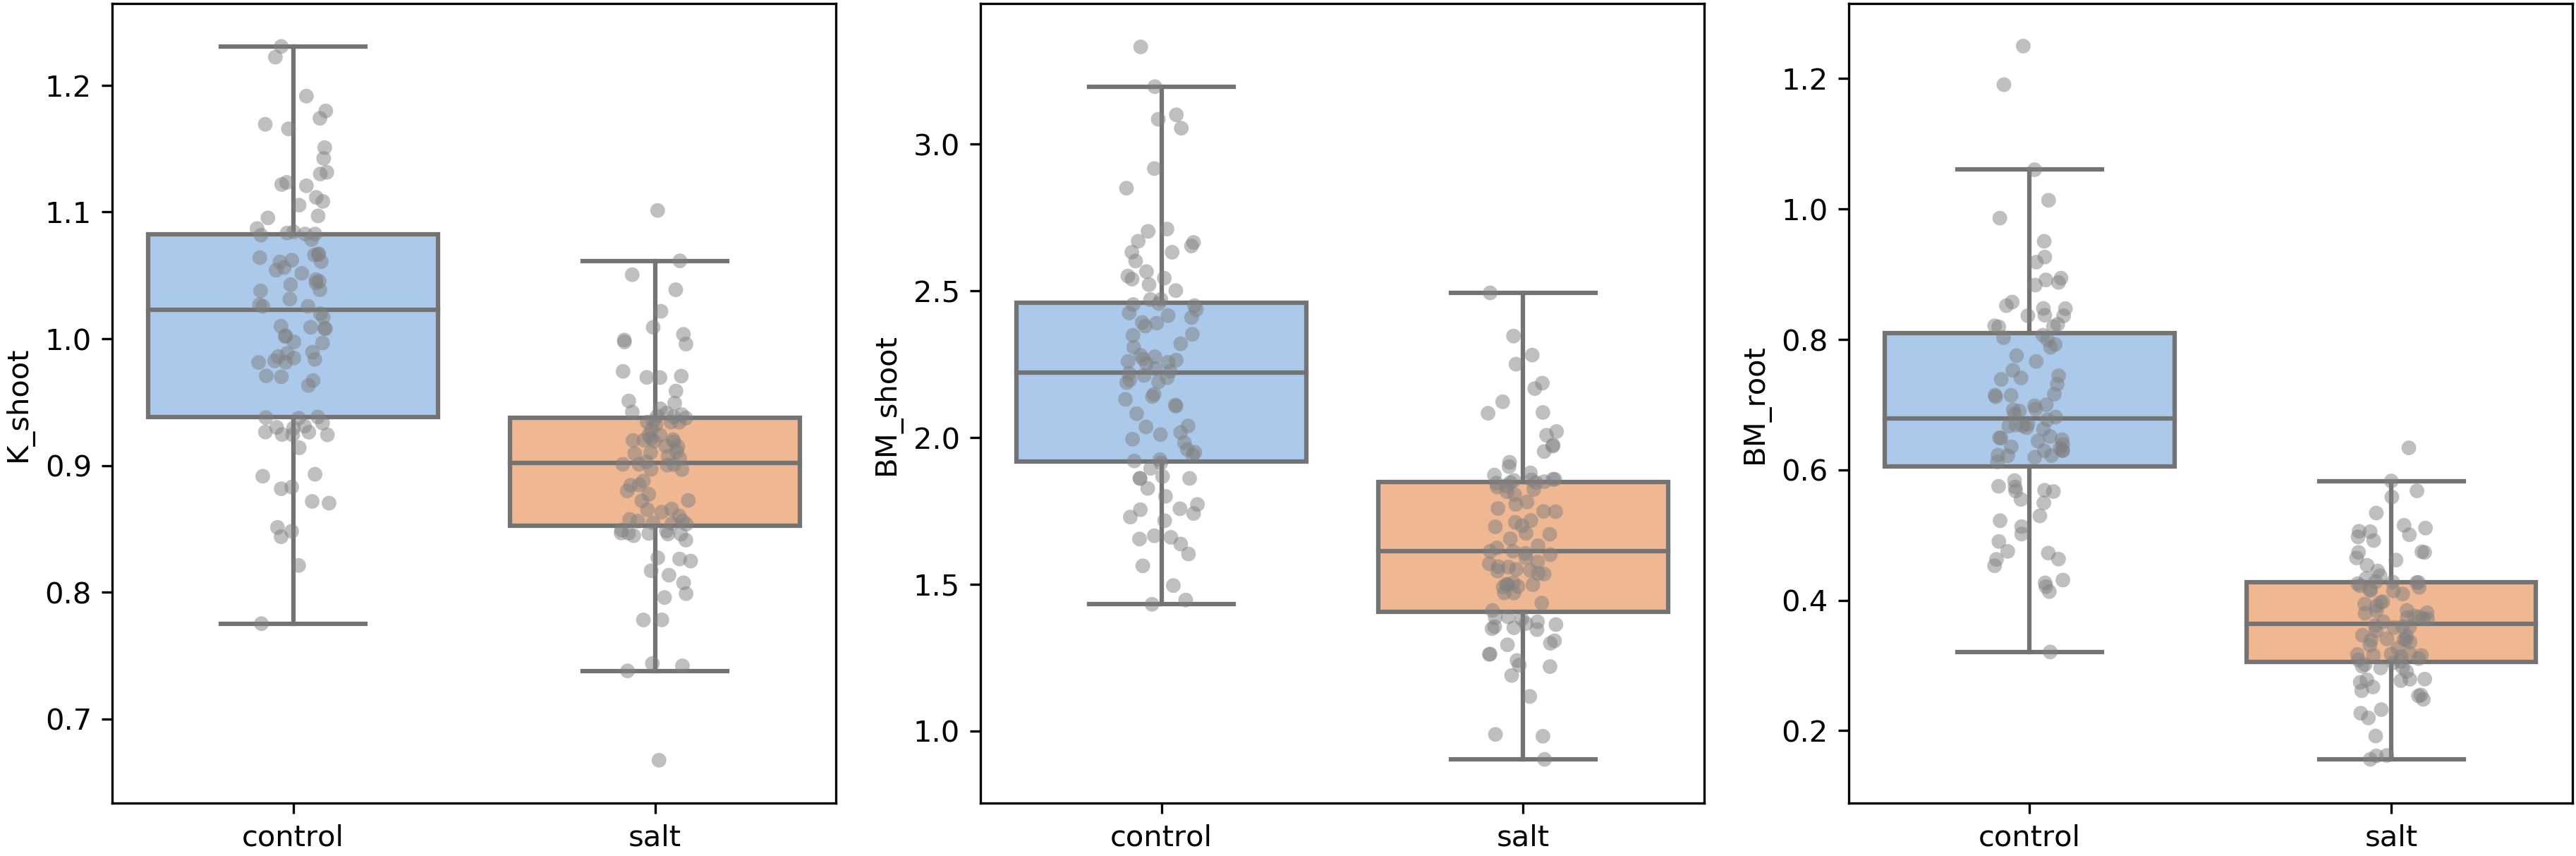
\includegraphics[clip,width=1\textwidth]{figures/phenotypic_traits.png}
  \caption{Phenotipic traits distribution under control and salt stress.}
  \label{fig:pdata}
\end{figure}

Using the affiliation matrix $F$ derived from the HLC output and the
Log Fold Change matrix $L_1$, a matrix $M$ is built by computing the
egengene for each of the $c = 5143$ modules. The LASSO technique is
applied by using each of the phenotypic traits as the outcome
variable, one at a time. As shown in Figure~\ref{fig:cross-val},
cross-validation is performed for each phenotypical trait in order to
select the corresponding regularization parameter $\lambda$ that
minimizes the mean-squared error.

\begin{figure}[htpb]
  \centering
  \subfloat[$K$ shoot, $\lambda = 0.013$]{%
    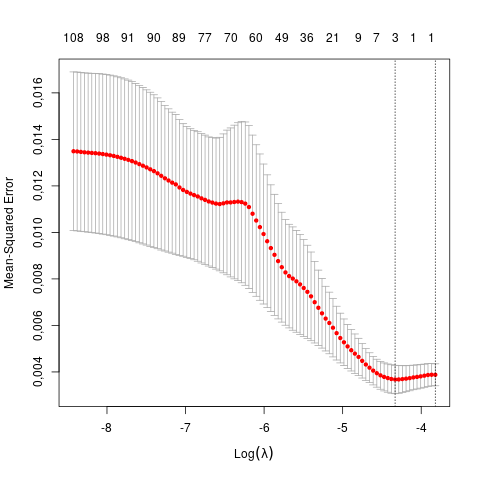
\includegraphics[width=0.33\textwidth]{figures/lambda_kshoot_2.png}
    \label{fig:lambda_kshoot}
  }
  \subfloat[Shoot biomass, $\lambda = 0.025$]{%
    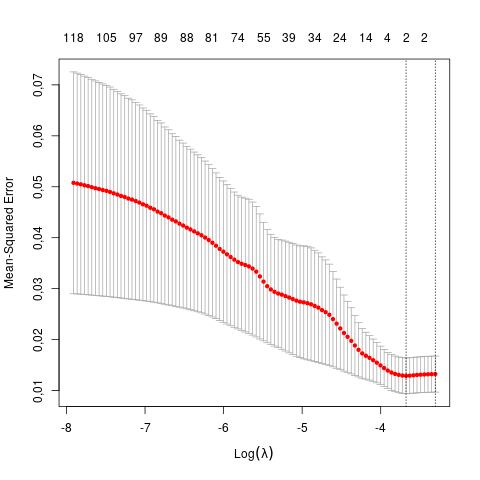
\includegraphics[width=0.33\textwidth]{figures/lambda_BMshoot_2.png}
    \label{fig:lambda_BMshoot}
  }
  \subfloat[Root biomass, $\lambda = 0.035$]{%
    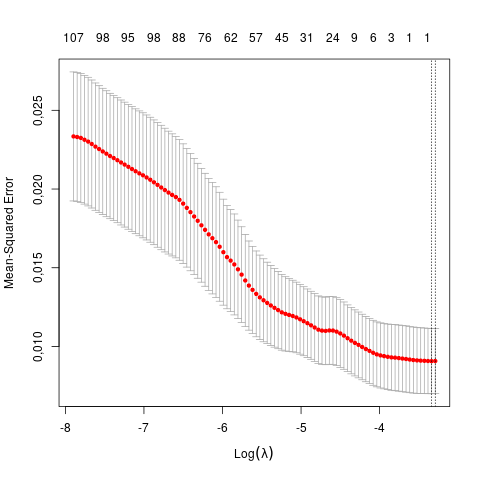
\includegraphics[width=0.33\textwidth]{figures/lambda_BMroot.png}
    \label{fig:lambda_BMroot}
  }
  \caption{Cross-validation of the LASSO regularization parameter
    $\lambda$, for each phenotypic trait.}
  \label{fig:cross-val}
\end{figure}

Finally, three LASSO models are adjusted by using the corresponding
$\lambda$ and phenotypical data with the egengens of matrix $M$. As
result, 6 modules are detected as relevant in the response to salt
stress in rice: 3 modules of 3 genes, each associated with shoot
$K$ content; 2 modules of 3 genes associated with shoot biomass; and 1
module of 4 genes associated with root biomass.

\subsection{Gene enrichment}

From the $19$ genes selected by LASSO, all but $3$ genes (the ones associated to $K$ content), are also identified as deferentially expressed ($|\ell_{ij}| \geq 2$) for at least one of the $92$ accessions. This suggest that those genes are strong candidates as stress responsive genes to salt conditions in rice. According to the Quickgo database, only $2$ of the $16$ diferentially expressed genes (both from the module related with shoot biomass) are named and have an associated protein product: Spermidine hydroxycinnamoyltransferase 2 (SHT2) and Lipoxygenase. Figure~\ref{fig:3d} shows their corresponding 3D protein structures.

% Figure 3d protein strucures
\begin{figure}[hptb]
  \centering
  \subfloat[Spermidine hydroxycinnamoyltransferase 2]{%
    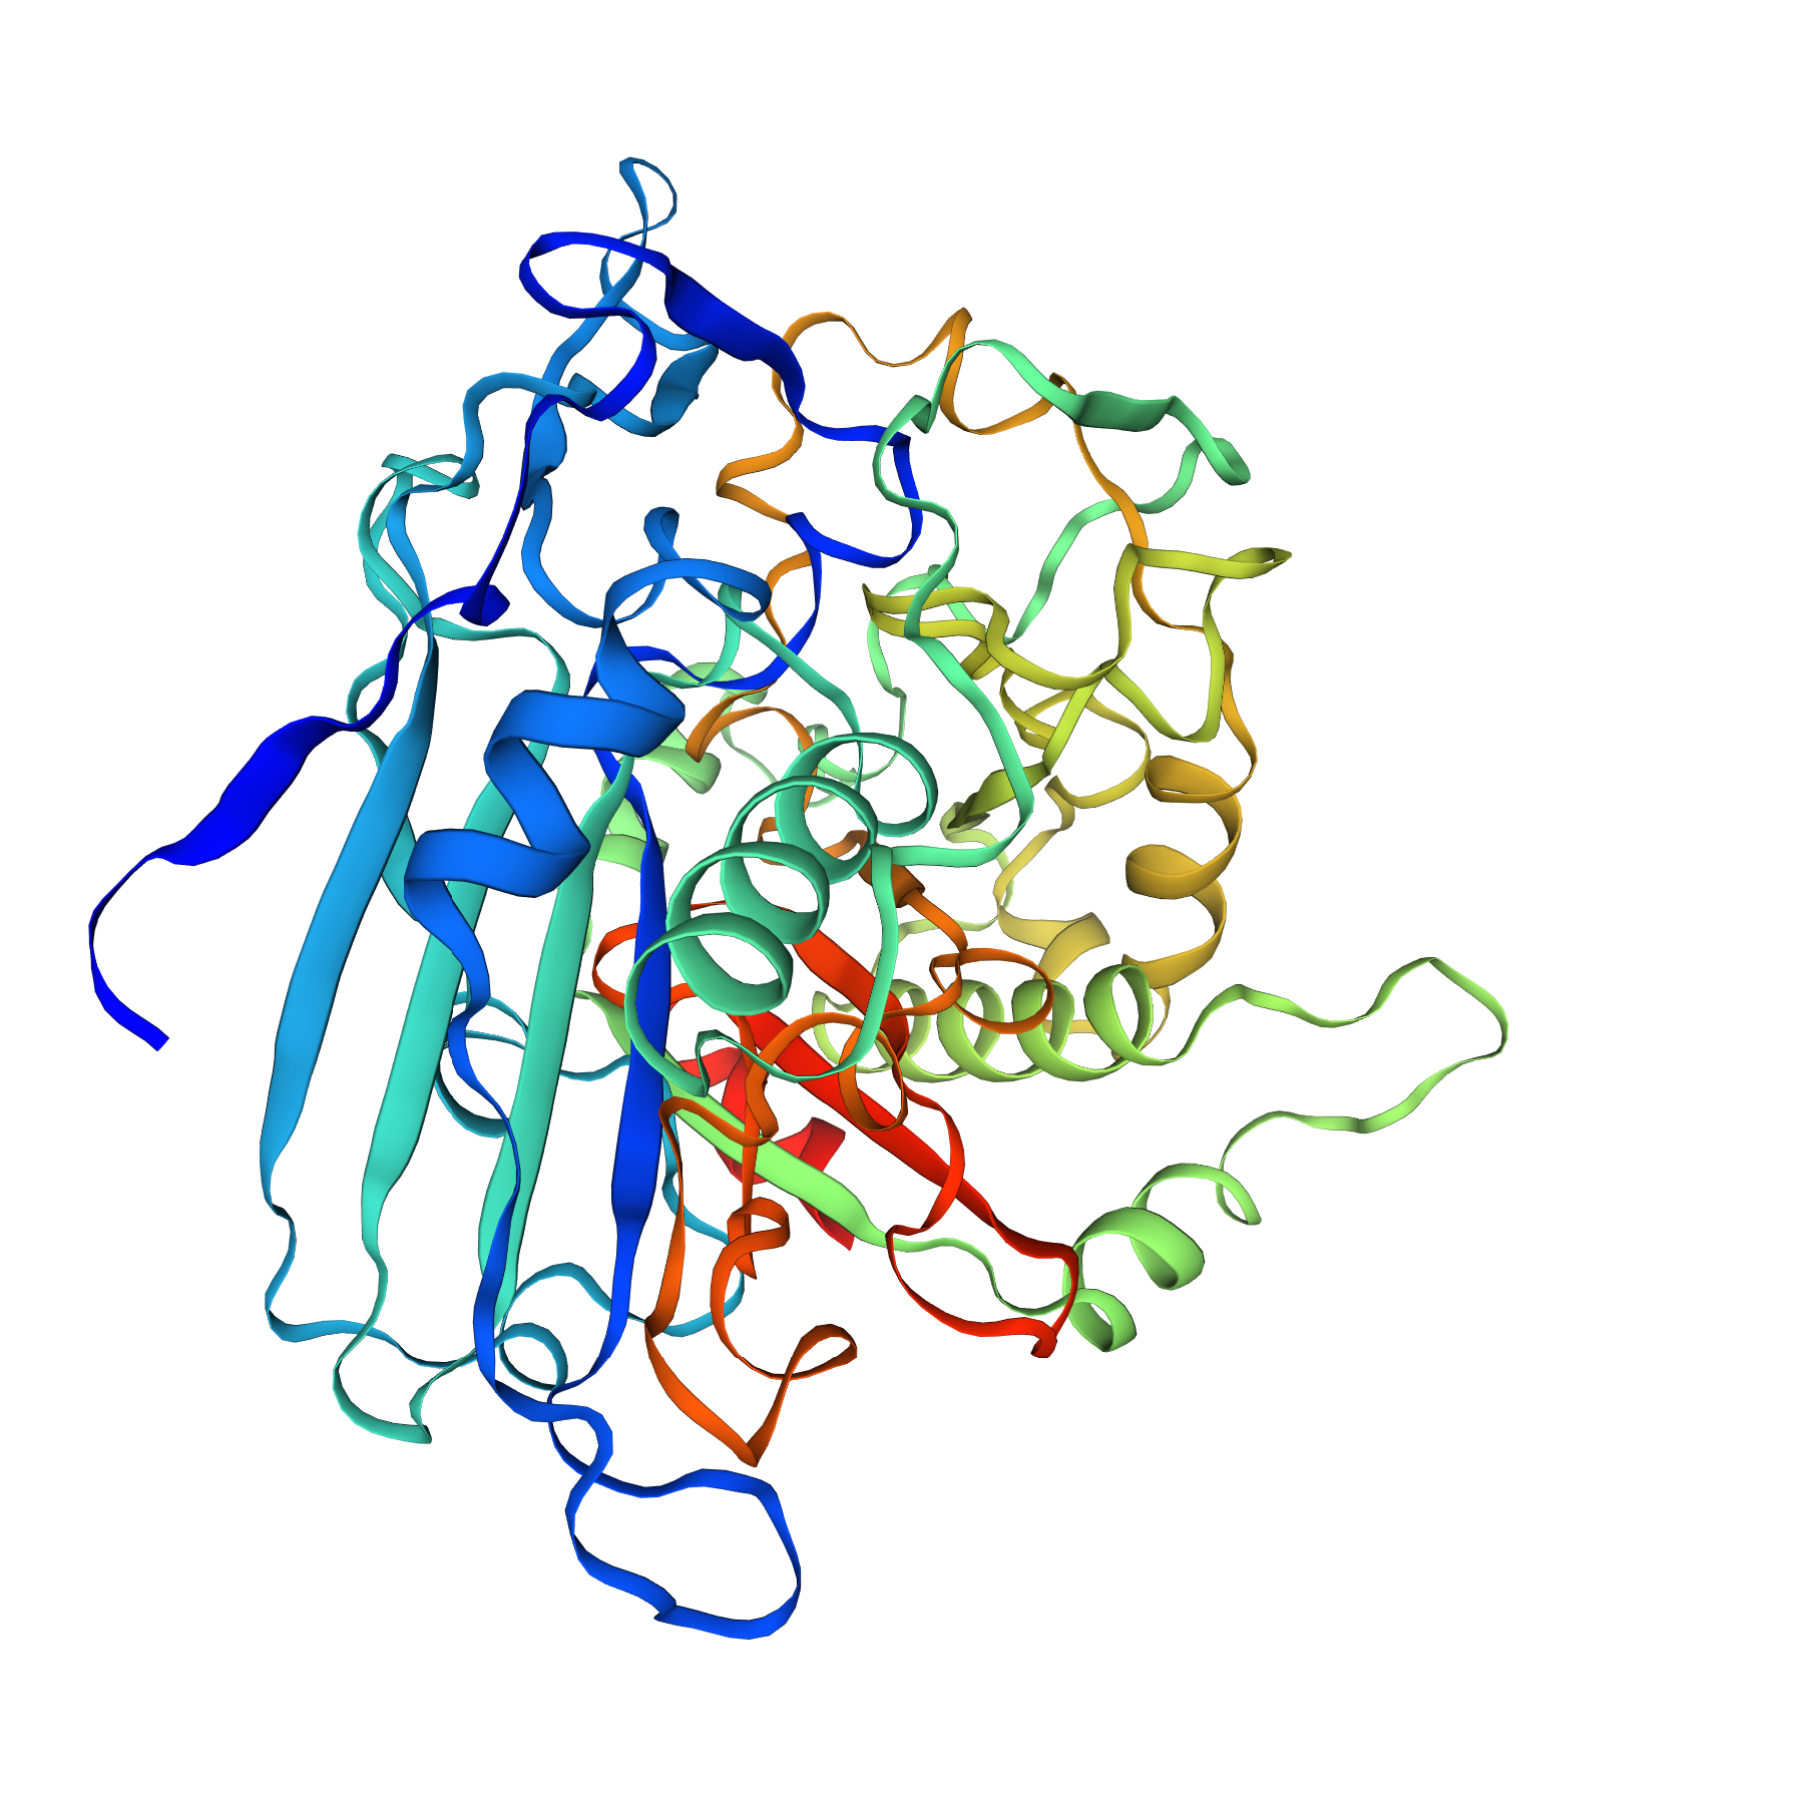
\includegraphics[width=0.45\textwidth]{figures/structure_LOC_Os12g27254.png}
    \label{fig:structure_SHT2}
  }\hfill
  \subfloat[Lipoxygenase]{%
    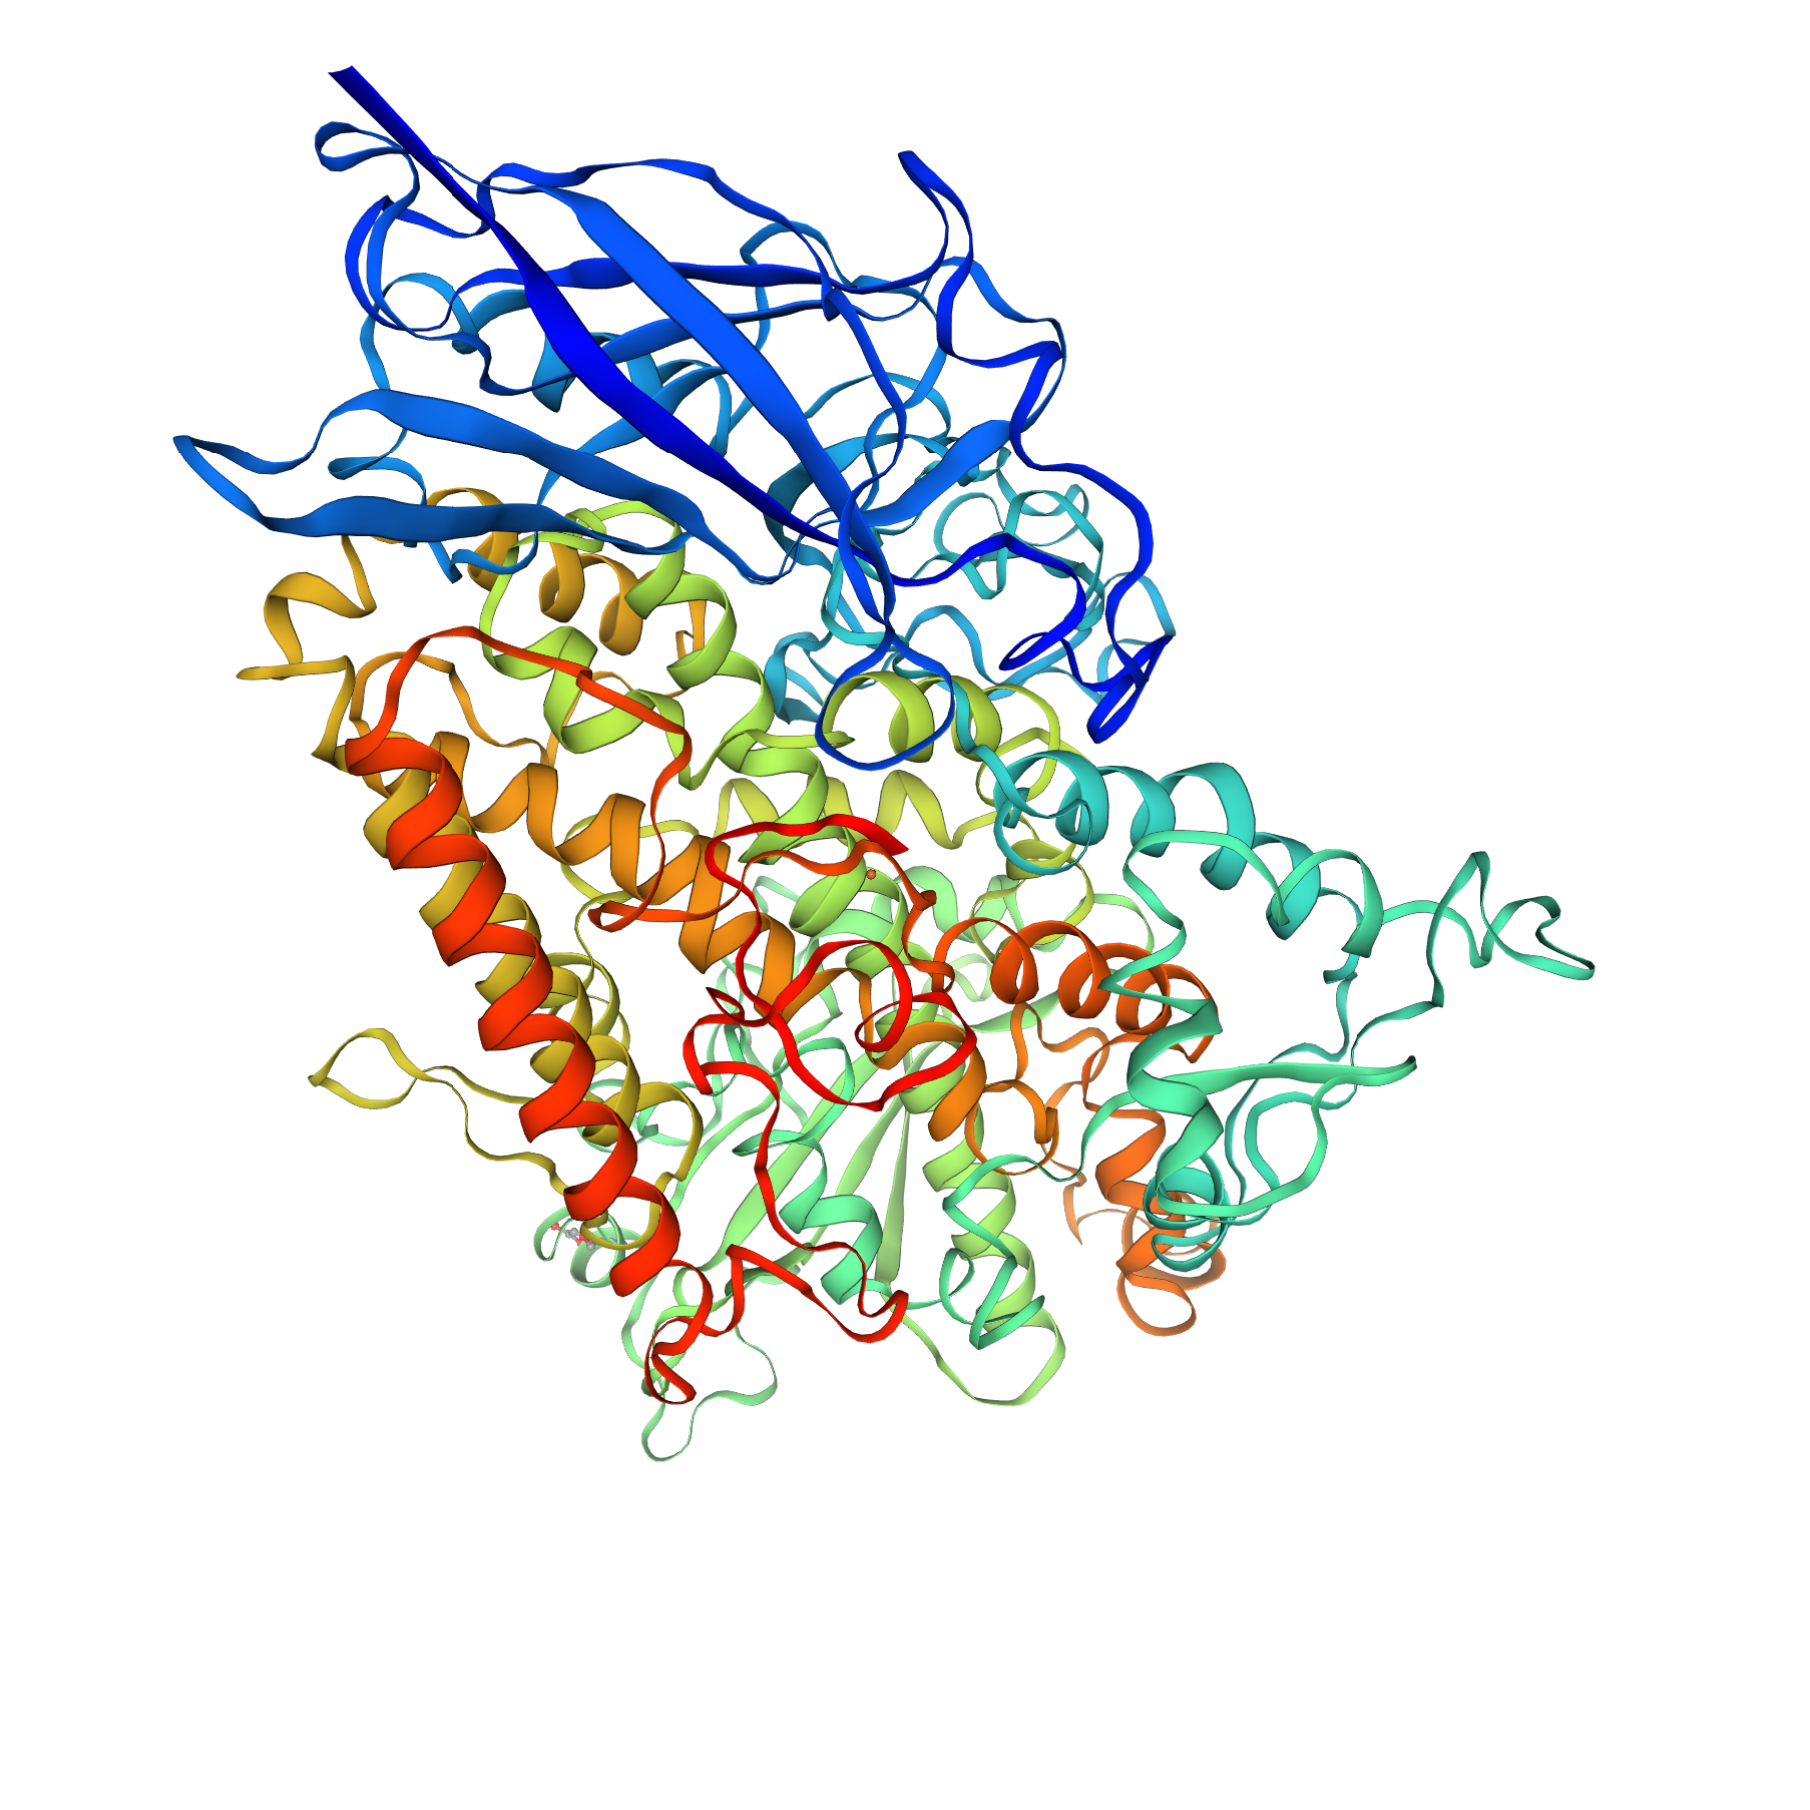
\includegraphics[width=0.45\textwidth]{figures/structure_LOC_Os12g37260.png}
    \label{fig:structure_Lipoxygenase}
  }
  \caption{3D protein structure of named genes selected by LASSO, available from~\cite{szklarczyk2016string}.}
  \label{fig:3d}
\end{figure}

Uniprot database~\cite{uniprot2018uniprot} reports, on the one hand,
that SHT2 contributes to the natural variation of spermidine-based
phenolamides in rice cultivars. On the other hand, it is reported that
plant lipoxygenase may be involved in a number of diverse aspects of
plant physiology including growth and development, pest resistance,
and senescence or responses to wounding~\cite{uniprot2018uniprot}. This protein is involved in
the pathway oxylipin biosynthesis, which is part of Lipid
metabolism. Aditionally, previous studies
%
in~\cite{gupta2013plant,hou2015persimmon,mittova2002salt,peng2019novel,roychoudhury2011amelioration}
%
provide evidence of biological implications of sperimidine and
lipoxygenase in tolerance to salt stress in other plants or even in
rice cultivars. However, further studies are needed to elucidate the
detailed biological function of the remaining 14 genes that have not
been named so far, which may have a potential relevance in stress
responsive mechanisms to salt conditions in rice.
